\documentclass{article}
\usepackage[english]{babel}
\usepackage{meta-inf/lib/naproche}
\documentclass[12pt,oneside]{book}

\usepackage[foundations]{../../lib/tex/naproche}
\usepackage{../../lib/tex/libraries}
\usepackage{graphicx}
\usepackage{float}
\usepackage{caption}
\usepackage{footnote}

\makesavenoteenv{tabular} % Make footnotes work in tabular environments


\title{Foundations of Mathematics}
\author{Marcel Schütz}
\date{2022}

\begin{document}
  \maketitle

  \tableofcontents

  \begin{figure}[H]
    \centering
    \fbox{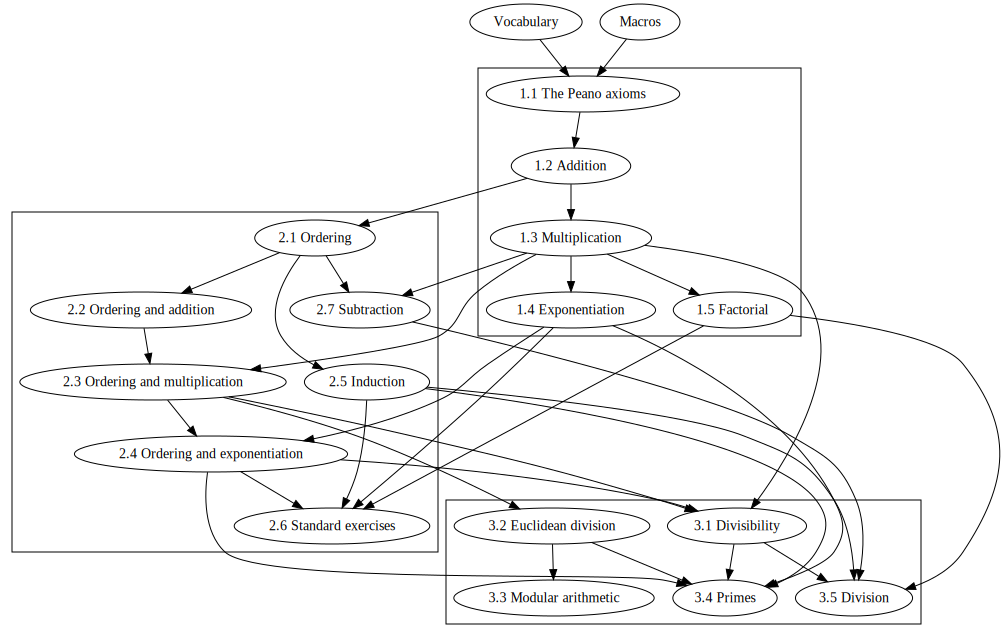
\includegraphics[width=0.9\linewidth]{./dependency-graph/graph.png}}
    \caption*{Interdependencies of the chapters}
  \end{figure}


  \section*{Introduction}

  This is a library providing a foundation of mathematics based on a
  Kelley-Morse like class theory with urelements.
  It introduces common operations on classes like unions or intersections
  (\cref{chapter:classes}) together with detailed proofs of their algebraic
  properties (\cref{chapter:computation-laws-for-classes}), the symmetric
  difference of two classes (\cref{chapter:symmetric-difference}) and the
  notions of ordered pairs and Cartesian products
  (\cref{chapter:pairs-and-products}) as well as proofs of the algebraic
  properties of the latter (\cref{chapter:computation-laws-for-products}).
  Moreover, it provides common operations on maps (\cref{chapter:maps}), various
  properties of images and preimages (\cref{chapter:image-and-preimage}) and the
  notions of injectivity, surjectivity, bijectivity
  (\cref{chapter:injections-surjections-bijections}) and invertibility of maps
  (\cref{chapter:invertible-maps}).
  The library provides an axiom system characterizing sets (\cref{chapter:sets})
  and, furthermore, it covers the notions of binary relations
  (\cref{chapter:binary-relations}), fixed-points of subset preserving maps
  (\cref{chapter:fixed-points}), including and equinumerosity
  (\cref{chapter:equinumerosity}).

  As two famous results it includes the Knaster-Tarski fixed point theorem
  (\cref{FOUNDATIONS_12_8420450166112256}) and the Cantor-Schröder-Bernstein
  theorem (\cref{FOUNDATIONS_13_1913663275401216}).

  \paragraph*{Usage.}
  At the very beginning of each chapter you can find the name of its source
  file, e.g. \path{foundations/sections/01_classes.ftl.tex} for
  \cref{chapter:classes}. This filename can be used to import the chapter via
  \Naproche's \texttt{readtex} instruction to another ForTheL text, e.g.:
  \begin{center}
    \verb`[readtex \path{foundations/sections/01_classes.ftl.tex}]`
  \end{center}

  \paragraph*{Checking times.}
  The checking times for each of the chapters may vary from computer to
  computer, but on mid-range hardware they are likely to be similar to those
  given in table below:

  \begin{center}
    \begin{tabular}{c|c|c}

      & \multicolumn{2}{c}{\textbf{Checking time}}
      \\
      \textbf{Chapter}
      & \textbf{without dependencies}     & \textbf{with dependencies}
      \\ \hline
      \ref{chapter:classes}
      & 00:04 min                         & 00:04 min
      \\
      \ref{chapter:computation-laws-for-classes}
      & 00:12 min                         & 00:16 min
      \\
      \ref{chapter:symmetric-difference}
      & 00:32 min                         & 00:48 min
      \\
      \ref{chapter:pairs-and-products}
      & 00:08 min                         & 00:12 min
      \\
      \ref{chapter:computation-laws-for-products}
      & 01:36 min                         & 01:56 min
      \\
      \ref{chapter:maps}
      & 01:13 min                         & 01:25 min
      \\
      \ref{chapter:image-and-preimage}
      & 01:28 min                         & 02:53 min
      \\
      \ref{chapter:injections-surjections-bijections}
      & 00:38 min                         & 02:03 min
      \\
      \ref{chapter:invertible-maps}
      & 02:20 min                         & 04:23 min
      \\
      \ref{chapter:sets}
      & 02:17 min                         & 06:40 min
      \\
      \ref{chapter:binary-relations}
      & 00:14 min                         & 06:54 min
      \\
      \ref{chapter:fixed-points}
      & 00:33 min                         & 07:13 min
      \\
      \ref{chapter:equinumerosity}
      & 01:48 min                         & 09:01 min
    \end{tabular}
  \end{center}


  \subfile{sections/01_classes.ftl.tex}
  \subfile{sections/02_computation-laws-for-classes.ftl.tex}
  \subfile{sections/03_symmetric-difference.ftl.tex}
  \subfile{sections/04_pairs-and-products.ftl.tex}
  \subfile{sections/05_computation-laws-for-products.ftl.tex}
  \subfile{sections/06_maps.ftl.tex}
  \subfile{sections/07_image-and-preimage.ftl.tex}
  \subfile{sections/08_injections-surjections-bijections.ftl.tex}
  \subfile{sections/09_invertible-maps.ftl.tex}
  \subfile{sections/10_sets.ftl.tex}
  \subfile{sections/11_binary-relations.ftl.tex}
  \subfile{sections/12_fixed-points.ftl.tex}
  \subfile{sections/13_equinumerosity.ftl.tex}
\end{document}


\usepackage[backend=bibtex]{biblatex}
\usepackage{csquotes}
\addbibresource{meta-inf/lib/bibliography}

\usepackage[
  type=CC,
  modifier=by-nc-sa,
  version=4.0,
]{doclicense}

\title{The Knaster-Tarski fixed point theorem and \\
the Cantor-Schröder-Bernstein Theorem}
\author{\Naproche formalization: \vspace{0.5em} \\
Alexander Holz, Marcel Schütz}
\date{2024}

\begin{document}
  \maketitle

  \noindent This is a formalization of the \textit{Knaster-Tarski Fixed Point
  Theorem} (i.e. of the assertion that every subset-preserving map has a fixed
  point) and of the \textit{Cantor-Schröder-Bernstein Theorem} (i.e. of the
  fact that two sets are equinumerous iff they can be embedded into each other),
  where the proof of the latter theorem is based on the former one, as in
  \cite{Schroeder2012}.

  \begin{imports}
    \begin{forthel}
      %[prove off][check off]
      [readtex \path{libraries/source/foundations/equinumerosity.ftl.tex}]
      [readtex \path{libraries/source/foundations/maps-and-systems-of-sets.ftl.tex}]
      [readtex \path{libraries/source/set-theory/zf.ftl.tex}]
      %[prove on][check on]
    \end{forthel}
  \end{imports}


  \section*{The Knaster-Tarski Fixed Point Theorem}

  \begin{forthel}
    \begin{theorem*}[Knaster-Tarski]\label{knaster_tarski}
      Let $x$ be a set.
      Let $h$ be a map from $\pow(x)$ to $\pow(x)$ that preserves subsets.
      Then $h$ has a fixed point.
    \end{theorem*}
    \begin{proof}
      (1) Define $A = \{y \in \pow(x) \mid y \subseteq h(y)\}$.
      Then $A$ is a subset of $\pow(x)$.
      We have $\bigcup A \in \pow(x)$.

      Let us show that (2) $\bigcup A \subseteq h(\bigcup A)$.
        Let $u \in \bigcup A$.
        Take $y \in A$ such that $u \in y$.
        Then $u \in h(y)$.
        We have $y \subseteq \bigcup A$.
        Hence $h(y) \subseteq h(\bigcup A)$.
        Indeed $h$ is a subset preserving map between systems of sets and $y, \bigcup A \in \dom(h)$.
        Thus $h(y) \subseteq h(\bigcup A)$.
        Therefore $u \in h(\bigcup A)$.
      End.

      Then $h(\bigcup A) \in A$ (by 1).
      Indeed $h(\bigcup A) \subseteq x$.
      (3) Hence $h(\bigcup A) \subseteq \bigcup A$.
      Indeed every element of $h(\bigcup A)$ is an element of some element of
      $A$.

      Thus $h(\bigcup A) = \bigcup A$ (by 2, 3).
    \end{proof}
  \end{forthel}


  \section*{The Cantor-Schröder-Bernstein Theorem}

  \begin{forthel}
    \begin{theorem*}[Cantor-Schröder-Bernstein]\label{cantor_schroeder_bernstein}
      Let $x,y$ be sets.
      $x$ and $y$ are equinumerous iff there exists a injective map from $x$ to $y$ and there exists an injective map from $y$ to $x$.
    \end{theorem*}
    \begin{proof}
      Case $x$ and $y$ are equinumerous.
        Take a bijection $f$ between $x$ and $y$.
        Then $f^{-1}$ is a bijection between $y$ and $x$.
        Hence $f$ is an injective map from $x$ to $y$ and $f^{-1}$ is an
        injective map from $y$ to $x$.
      End.

      Case there exists an injective map from $x$ to $y$ and there exists an injective map from $y$ to $x$.
        Take an injective map $f$ from $x$ to $y$.
        Take an injective map $g$ from $y$ to $x$.
        We have $y \setminus f[a] \subseteq y$ for any $a \in \pow(x)$.

        (1) Define $h(a) = x \setminus g[y \setminus f[a]]$ for $a \in \pow(x)$.

        $h$ is a map from $\pow(x)$ to $\pow(x)$.
        Indeed $h(a)$ is a subset of $x$ for each subset $a$ of $x$.

        Let us show that $h$ preserves subsets.
          Let $u, v$ be subsets of $x$.
          Assume $u \subseteq v$.
          Then $f[u] \subseteq f[v]$.
          Hence $y \setminus f[v] \subseteq y \setminus f[u]$.
          Thus $g[y \setminus f[v]] \subseteq g[y \setminus f[u]]$.
          Indeed $y \setminus f[v]$ and $y \setminus f[u]$ are subsets of $y$.
          Therefore $x \setminus g[y \setminus f[u]] \subseteq x \setminus g[y \setminus f[v]]$.
          Consequently $h[u] \subseteq h[v]$.
        End.

        Hence we can take a fixed point $c$ of $h$ (by \nameref{knaster_tarski}).

        (2) Define $F(u) = f(u)$ for $u \in c$.

        We have $c = h(c)$ iff $x \setminus c = g[y \setminus f[c]]$.
        $g^{-1}$ is a bijection between $\range(g)$ and $y$.
        Thus $x \setminus c = g[y \setminus f[c]] \subseteq \range(g)$.
        Therefore $x \setminus c$ is a subset of $\dom(g^{-1})$.

        (3) Define $G(u) = g^{-1}(u)$ for $u \in x \setminus c$.

        $F$ is a bijection between $c$ and $\range(F)$.
        $G$ is a bijection between $x \setminus c$ and $\range(G)$.

        Define \[ H(u) =
          \begin{cases}
            F(u) & : u \in c \\
            G(u) & : u \notin c
          \end{cases} \]
        for $u \in x$.

        Let us show that $H$ is a map to $y$.
          $\dom(H)$ is a set and every value of $H$ is an object.
          Hence $H$ is a map.

          Let us show that every value of $H$ lies in $y$.
            Let $v$ be a value of $H$.
            Take $u \in x$ such that $H(u) = v$.
            If $u \in c$ then $v = H(u) = F(u) = f(u) \in y$.
            If $u \notin c$ then $v = H(u) = G(u) = g^{-1}(u) \in y$.
          End.
        End.

        (4) $H$ is surjective onto $y$.
        Indeed we can show that every element of $y$ is a value of $H$.
          Let $v \in y$.

          Case $v \in f[c]$.
            Take $u \in c$ such that $f(u) = v$.
            Then $F(u) = v$.
          End.

          Case $v \notin f[c]$.
            Then $v \in y \setminus f[c]$.
            Hence $g(v) \in g[y \setminus f[c]]$.
            Thus $g(v) \in x \setminus h(c)$.
            We have $g(v) \in x \setminus c$.
            Therefore we can take $u \in x \setminus c$ such that $G(u) = v$.
            Then $v = H(u)$.
          End.
        End.

        (5) $H$ is injective.
        Indeed we can show that for all $u, v \in x$ if $u \neq v$ then $H(u) \neq H(v)$.
          Let $u,v \in x$.
          Assume $u \neq v$.

          Case $u,v \in c$.
            Then $H(u) = F(u)$ and $H(v) = F(v)$.
            We have $F(u) \neq F(v)$.
            Hence $H(u) \neq H(v)$.
          End.

          Case $u,v \notin c$.
            Then $H(u) = G(u)$ and $H(v) = G(v)$.
            We have $G(u) \neq G(v)$.
            Hence $H(u) \neq H(v)$.
          End.

          Case $u \in c$ and $v \notin c$.
            Then $H(u) = F(u)$ and $H(v) = G(v)$.
            Hence $v \in g[y \setminus F[c]]$.
            We have $G(v) = g^{-1}(v) \in y \setminus F[c]$.
            Indeed $v = g(v') for some v' \in y \setminus F[c]$.
            Thus $G(v) \neq F(u)$.
          End.

          Case $u \notin c$ and $v \in c$.
            Then $H(u) = G(u)$ and $H(v) = F(v)$.
            Hence $u \in g[y \setminus F[c]]$.
            We have $G(u) = g^{-1}(u) \in y \setminus F[c]$.
            Indeed $u = g(u') for some u' \in y \setminus F[c]$.
            Thus $G(u) \neq F(v)$.
          End.
        End.

        Consequently $H$ is a bijection between $x$ and $y$ (by 4, 5).
        Therefore $x$ and $y$ are equinumerous.
      End.
    \end{proof}
  \end{forthel}

  \printbibliography

  \section*{Copyright}
  \doclicenseThis
\end{document}
